\subsection*{Fundamental: Hierarchy of Roles\label{sec:hierarchy-of-roles}}

Inclusion of hierarchy in the section on Fundamentals of Bureaucracy does not imply that hierarchy is a required feature of bureaucracy. Hierarchies of bureaucrats are a conventional \href{https://en.wikipedia.org/wiki/Organizational_structure}{organizational structure}
\index{Wikipedia!organizational structure@\href{https://en.wikipedia.org/wiki/Organizational_structure}{organizational structure}}%
%\iftoggle{WPinmargin}{\marginpar{$>$Wikipedia: Organizational structure}}{}%
and are worth studying even if not essential to bureaucracy. Understanding hierarchy is relevant to identifying recurring behavior and patterns to leverage.
Organizations of bureaucrats can intentionally work against the use of hierarchy for decisions, but the amount of effort needed to enable alternatives results in hierarchy being a common approach.

% Hierarchy is related to bureaucracy by the specialization of knowledge and delegation of decision authority.

Hierarchical decision-making is one option for coordination among alternatives (like consensus, voting, or dictatorship), so why is hierarchy so common? Members of an organization gravitate towards hierarchy because it helps define task scope, assigns responsibility, and obviates a need for building consensus. Reaching consensus or taking a vote for every decision would take time and be more burdensome than appointing a person as the decision-maker. At the other extreme, relying on a dictator decreases the value other stakeholders can contribute. There is a Pareto frontier of imperfect decision-making techniques when multiple stakeholders are involved. Some approaches require more time for the informaion gather to inform a decision, others take time due consensus, while other approaches take less time by involving fewer people but have poorer results from the decision.


The benefits of formal hierarchy include improved capacity for the number of policy decisions made, enabling consistency of decisions, and leveraging specialization of knowledge. 
Hierarchical decision-making has costs: higher latency (compared to a single decider), inconsistency among bureaucrats (dissemination isn't perfect), waste due to inefficiency,  
\hyperref[sec:unavoidable-hazards]{and others}
\marginpar{See page~\pageref{sec:unavoidable-hazards}.}%
like enabling strategic ignorance. Bureaucrats in positions of power can deny knowing of improper activity~\cite{2019_McGoey, 2012_McGoey}.  Whether that is a problem or benefit depends on your role. 

\subsubsection*{Why does Hierarchical Structure Arise in Organizations?}

In an ideal situation for managing access to a shared resource, one person would have sufficient depth of knowledge and breadth of information for decision-making. 
That might not be possible in every situation. One way to resolve this is to identify distinct scopes of responsibility and then assign different members of an organization separate scopes for decision-making. Within a decision-making scope there may be more work than one person can handle, so a team is formed. That team may have some members focused on tactical work and other members focused on coordination. 
Hierarchy within an organization is the formalization of separate decision-making scopes and associated specialization. 

Partitioning knowledge and decision-making enable complex work beyond what one person can do and causes friction among members. An expert reporting to a manager knows things the manager does not, and the manager may have context that the expert lacks. Both bureaucrats (the expert and the manager) need to convey their respective understanding and seek a holistic view.

\subsubsection*{Characterizing Hierarchy}

A conventional characterization of an organization's hierarchy involves two criteria: the depth and breadth of the \gls{org chart}.
The more people a supervisor oversees, the flatter the organization -- that's the breadth of the organization. The depth of the hierarchy is how many layers there are. See the Valve handbook~\cite{2012_Valve} and Joreen's essay~\cite{1972_Joreen} for contrasting views on the merits of an organization's hierarchy. 

Organizations that try to be flatter (more employees per manager) saturate the attention of managers. As a result there are more discussions that everyone has to pay attention to so they don't miss something happening. The opposite design (fewer employees per manager) is less noisy but results in silos of reporting because lateral coordination is more challenging.

Another view of an organization's hierarchy also involves two criteria. The two choices that shape hierarchy are how many people a supervisor oversees and  how many supervisors a person has. 
You might na\"ively expect that an employee has one boss, but that is \href{https://en.wikipedia.org/wiki/Matrix_management}{not a requirement}.%
\index{Wikipedia!matrix management@\href{https://en.wikipedia.org/wiki/Matrix_management}{Matrix management}}\iftoggle{WPinmargin}{\marginpar{$>$Wikipedia: Matrix management}}{}
A supervisor for a given topic may have many people reporting to them, and a bureaucrat with multiple roles may report to more than one supervisor.

%Another paradigm for characterizing hierarchies of humans is to identify roles for the participants. 

Often the concept of hierarchy intended to describe the relations in an organization is not representative of actual relationships among coworkers. For that reason, the concept of roles is another way to characterize interactions. Roles are defined by boundaries of responsibility in an organization. Similar to the motive for hierachy, the purpose of a role is to minimize conflict, decrease the need for coordination, reduce redundancy, and allow for control of resources. Clear boundaries of responsibility  enable effective bureaucracy. 

The structure of an organization is dynamic, but at each point in time an organization typically has a defined set of roles. Different scopes of decision authority distinguish each role. 
Roles are often confused with titles. What matters is the role (scope of decisions) and who reports to whom. The names of teams can be similarly not descriptive.

As part of your practice of Process Empathy, consider the roles and titles of bureaucrats you collaborate with and rely on. A person may have more roles than titles, and the two are loosely correlated. Your perception of another person's role may not match their self-perceived role. You can discuss these differences and better understand each person's expectations. 


\subsubsection*{Sequencing Dissemination of Information}

A hierarchical organization with partitioned knowledge introduces a challenge: the order in which you share information with others matters. Your choices for who to first describe an idea to are your peers, your management, and the people you manage. 
\marginpar{$>>$ Trilemma}% 
\index{trilemma!communication priority: peers, management, subordinates}%
The people you manage know more about the topic and are exposed to the consequences. Giving them a chance to vet the idea results in a more robust idea and validates their value in the organization. Alternatively, first sharing your idea with management  allows your superiors to provide context you might not be aware of. And choosing to  start the conversation with your peers first indicates you value the relationship and decreases the risk of duplicating work. There is no right answer. 


\subsubsection*{Autonomy in a Hierarchical Organization}

Acting as part of a group means ceding part of your autonomy. Hierarchy cedes some of your responsibility and adds expectations about relationships.
The consequence of hierarchy in an organization is that, as a member of the bureaucracy, you do not have full autonomy -- otherwise you would not be a member of the hierarchy. At the same time, you are not under strict control of the organization -- you still have some subjective %decision-making 
% 2023-01-11: Brian Black says to decrease redundancy
authority as a bureaucrat.


In a hierarchy, the upward flow of decision authority and justification is a feature, not a bug.
If justifications and decisions were bidirectional that would be consensus and take more time.

The person at the top of the hierarchy does not know everything. The person at the top of the hierarchy does not have input on every decision made in the organization. All members of the bureaucracy retain some autonomy.

The autonomy retained by members of a hierarchy can result in problems for participants. 
%* Hopping up the chain, skipping your immediate management
% Skip level meetings, which make  nervous 
One example is when a member seeks upward communication and skips engaging the person directly above them in the chain of command. A similar problem occurs in the opposite direction when a person higher up engages someone far below them without coordinating with the management between them. This is referred to as ``skip-level meetings'' by Grove in~\cite{1995_Grove}. In both these cases, neglecting to engage middle management risks missing relevant context necessary for effective communication. Middle managers can get nervous or frustrated when they aren't part of the conversation.

% * lateral meetings with your work cousins. 
Another challenge induced by hierarchy for nominally autonomous members is direct communication between lateral peers. If you think of a hierarchical organization using the labels a family tree, the members of your team are your siblings and the team manager is the parent. Talking with your peers on other teams is engaging with you cousins. When discussions with your professional work cousins is informal and ad hoc, that can disrupt the intended flow of coordination between your manager and the other team's manager. This can interfere with the focus and priorities of each team. 

Finally, the challenge for autonomous members is uncoordinated broadcasting of information to the entire hierarchical organization. Because each person lacks a holistic understanding of the complex organization, angst and misinterpretation can occur. The typical fix is to rely on upward and downward propagation of information in the chain of command. That way local context can be applied at each layer specific to the audience.

\subsubsection*{Roles Outside the Hierarchy}

Independent of the defined roles and formal titles in an organization's hierarchy, there are a set of implicit roles and a separate social hierarchy of informal influencers and decision-makers. Informal influencers in a bureaucracy usually have long relationships with the decision-maker, relevant credentials, or both. The credentials can be formal (e.g., a \href{https://en.wikipedia.org/wiki/Doctor_of_Philosophy}{PhD}) 
\index{Wikipedia!Doctor of Philosophy@\href{https://en.wikipedia.org/wiki/Doctor_of_Philosophy}{Doctor of Philosophy}}\iftoggle{WPinmargin}{\marginpar{$>$Wikipedia: Doctor of Philosophy}}{}
or informal (demonstrated success on a project). In either case, the decision-maker is relying on another person's expertise. 

Another set of informal relationships within an organization is between mentors and mentees. These relations allow mentors to share institutional knowledge with mentees and enable people in senior positions to access the novice perspective. 


\subsubsection*{Fear Induced by Hierarchy}

One consequence of hierarchy is a sense of fear felt by people who report to other people. This fear stems from the loss of control (less autonomy) that leaves the person feeling disempowered. 

For example, consider the following relationship. Sue is perceived to have power over another person, Amy, because Amy gave up some control to Sue. Amy's lack of control over decisions triggers the feeling of fear in Amy, regardless of how Sue behaves. (See Figure~\ref{fig:subordinate_and_supervisor}.) Having responsibility for decisions also induces anxiety.

\begin{figure}[H]
    \centering
    % left lower right upper
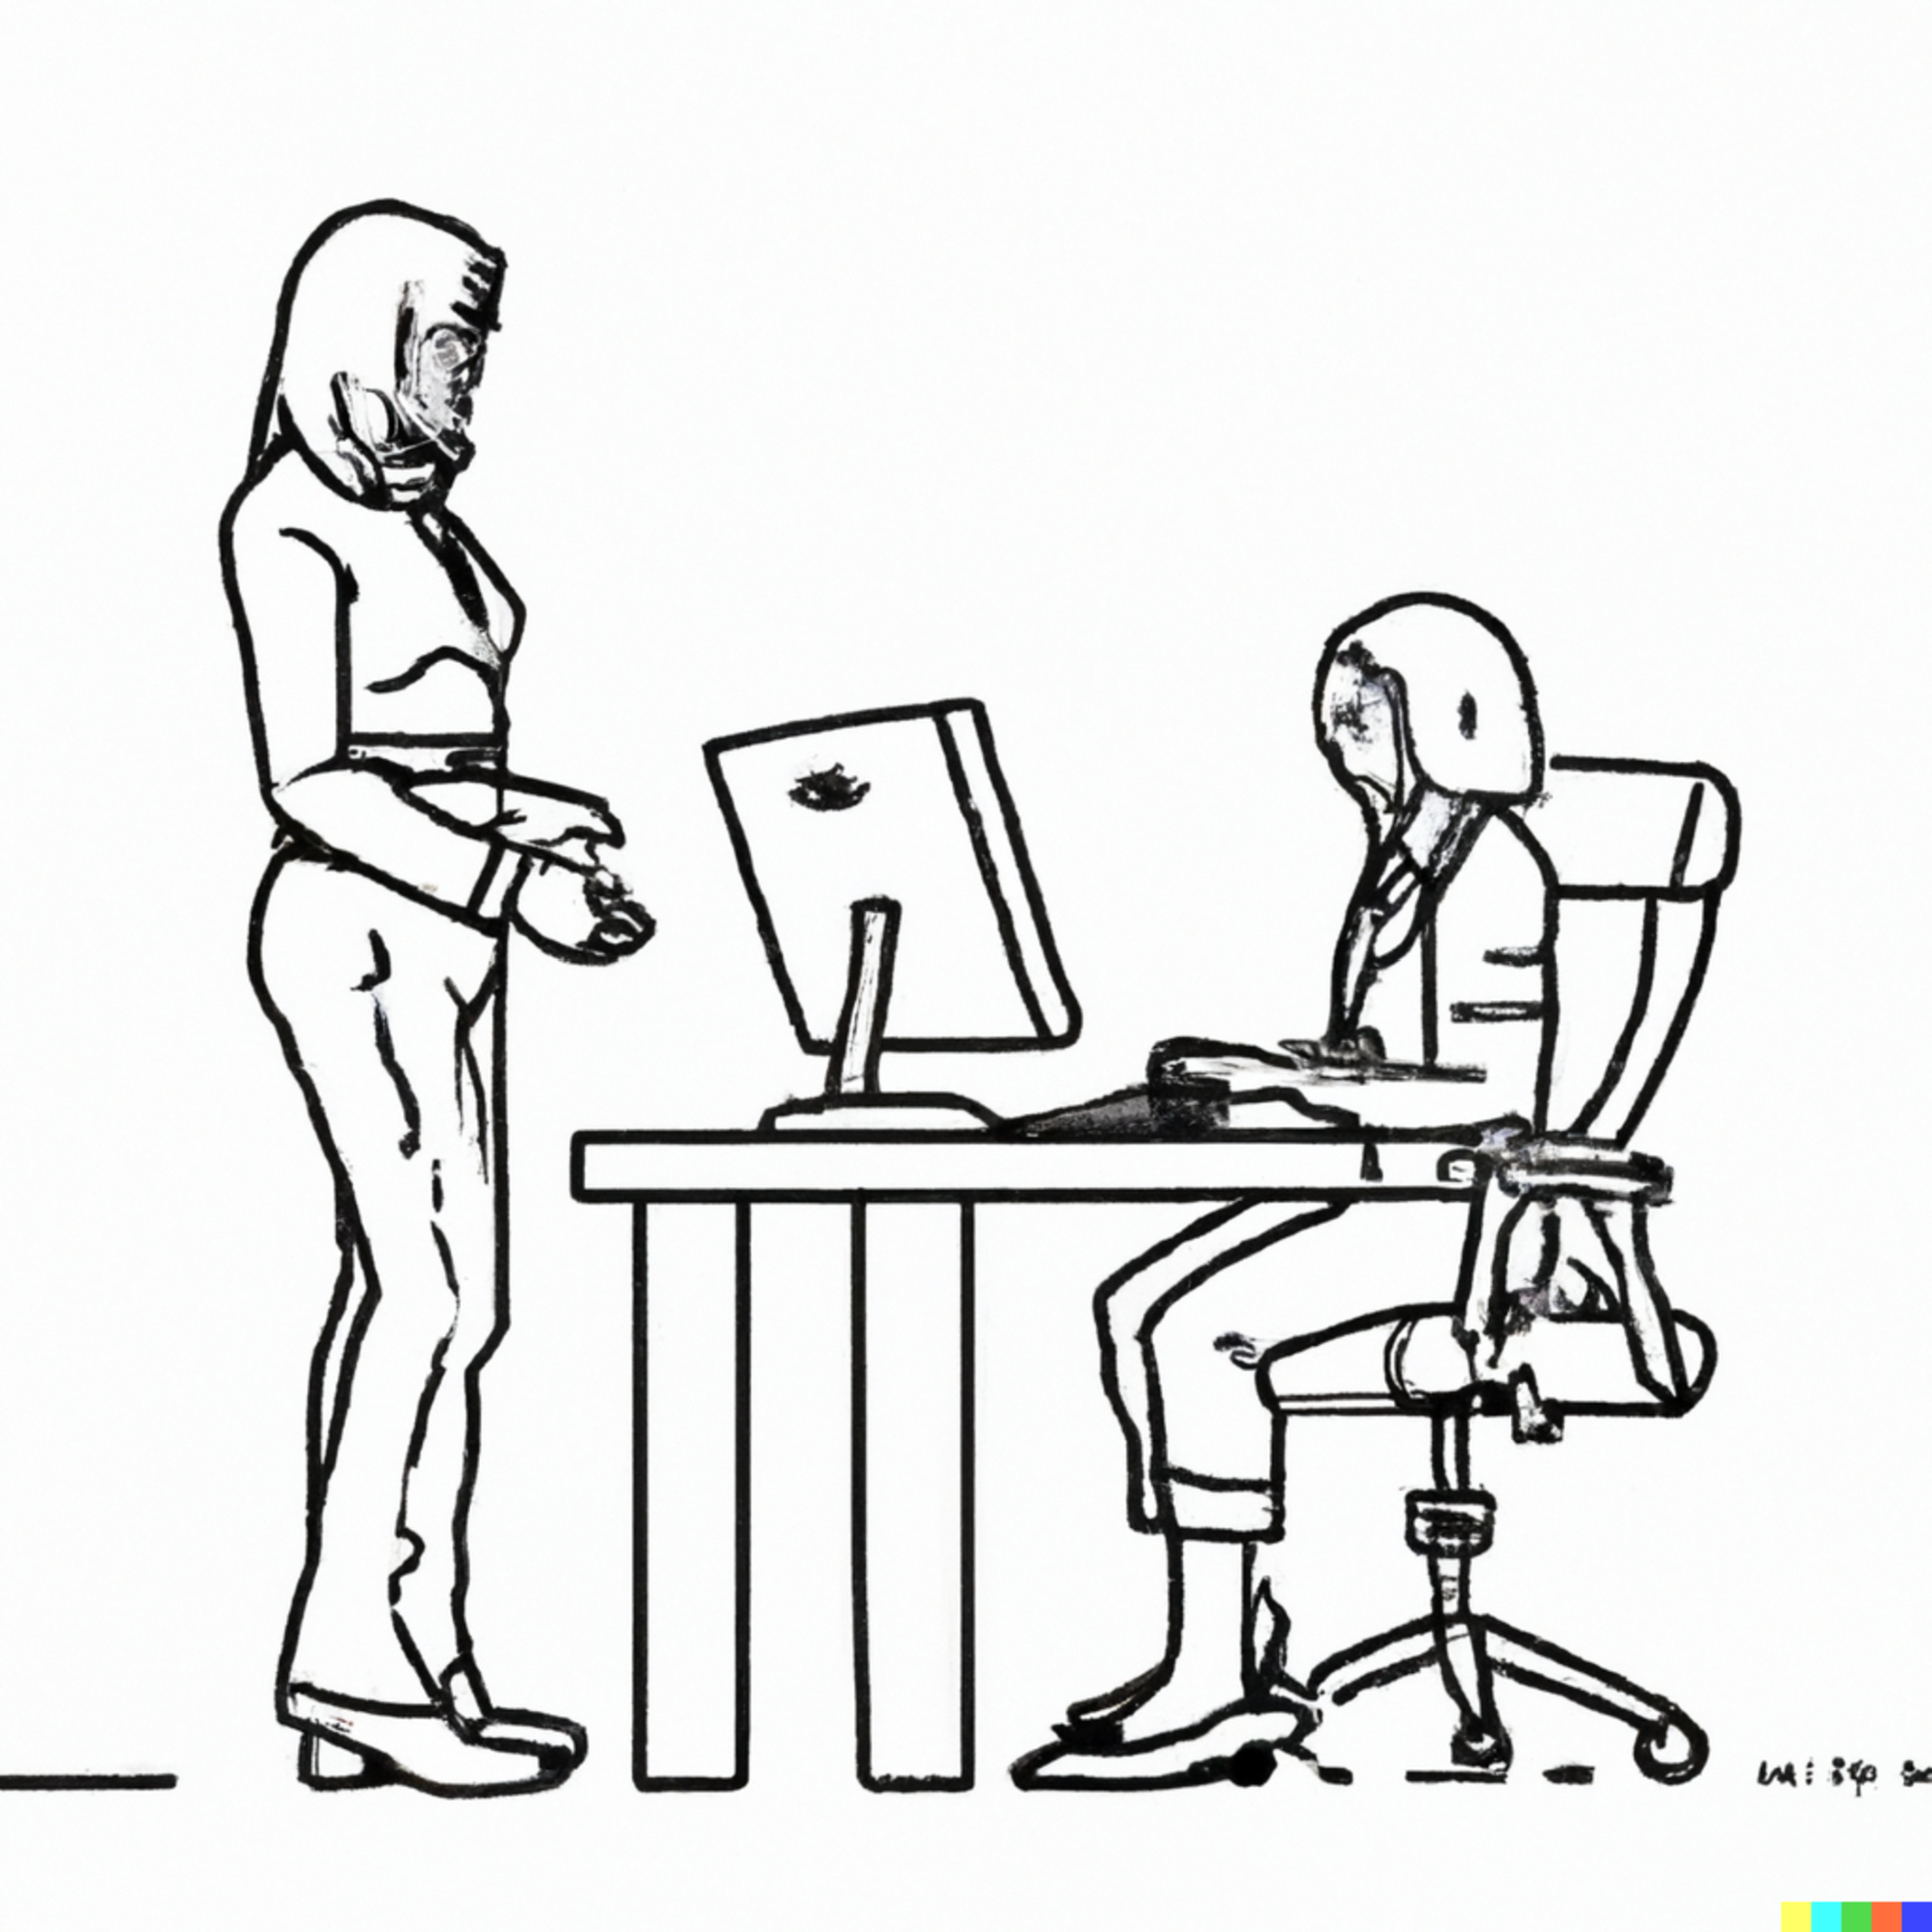
\includegraphics[width=0.6\textwidth,trim={0 1cm 0 0},clip]{images/female_supervisor_standing_while_talking_to_seated_female_employee_typing_on_keyboard.pdf}
    \caption{Sue and Amy discuss a work-related topic. The person with less perceived power can feel fear associated with loss of control.}
    \label{fig:subordinate_and_supervisor}
\end{figure}



If Sue is aware of the potential for this emotional experience, Sue can compensate for Amy's fear by being friendly and receptive towards Amy. Alternatively Sue may exploit or rely on the fear felt by the people she manages. Sue not noticing or accounting for Amy's fear does not invalidate Amy's emotional experience.


% Active bystander when the person doing wrong is in a position of authority
% PACT (Probe, Alert, Challenge, Take Action)
% https://mobile.twitter.com/GeorgetownABLE/status/1408498438203969541


% Mintzberg's Coordination Mechanisms
% https://www.youtube.com/watch?v=IZET8VjSifQ

